% Options for packages loaded elsewhere
\PassOptionsToPackage{unicode}{hyperref}
\PassOptionsToPackage{hyphens}{url}
%
\documentclass[
  10pt,
  ignorenonframetext,
]{beamer}
\usepackage{pgfpages}
\setbeamertemplate{caption}[numbered]
\setbeamertemplate{caption label separator}{: }
\setbeamercolor{caption name}{fg=normal text.fg}
\beamertemplatenavigationsymbolsempty
% Prevent slide breaks in the middle of a paragraph
\widowpenalties 1 10000
\raggedbottom
\setbeamertemplate{part page}{
  \centering
  \begin{beamercolorbox}[sep=16pt,center]{part title}
    \usebeamerfont{part title}\insertpart\par
  \end{beamercolorbox}
}
\setbeamertemplate{section page}{
  \centering
  \begin{beamercolorbox}[sep=12pt,center]{part title}
    \usebeamerfont{section title}\insertsection\par
  \end{beamercolorbox}
}
\setbeamertemplate{subsection page}{
  \centering
  \begin{beamercolorbox}[sep=8pt,center]{part title}
    \usebeamerfont{subsection title}\insertsubsection\par
  \end{beamercolorbox}
}
\AtBeginPart{
  \frame{\partpage}
}
\AtBeginSection{
  \ifbibliography
  \else
    \frame{\sectionpage}
  \fi
}
\AtBeginSubsection{
  \frame{\subsectionpage}
}
\usepackage{amsmath,amssymb}
\usepackage{lmodern}
\usepackage{iftex}
\ifPDFTeX
  \usepackage[T1]{fontenc}
  \usepackage[utf8]{inputenc}
  \usepackage{textcomp} % provide euro and other symbols
\else % if luatex or xetex
  \usepackage{unicode-math}
  \defaultfontfeatures{Scale=MatchLowercase}
  \defaultfontfeatures[\rmfamily]{Ligatures=TeX,Scale=1}
\fi
% Use upquote if available, for straight quotes in verbatim environments
\IfFileExists{upquote.sty}{\usepackage{upquote}}{}
\IfFileExists{microtype.sty}{% use microtype if available
  \usepackage[]{microtype}
  \UseMicrotypeSet[protrusion]{basicmath} % disable protrusion for tt fonts
}{}
\makeatletter
\@ifundefined{KOMAClassName}{% if non-KOMA class
  \IfFileExists{parskip.sty}{%
    \usepackage{parskip}
  }{% else
    \setlength{\parindent}{0pt}
    \setlength{\parskip}{6pt plus 2pt minus 1pt}}
}{% if KOMA class
  \KOMAoptions{parskip=half}}
\makeatother
\usepackage{xcolor}
\newif\ifbibliography
\setlength{\emergencystretch}{3em} % prevent overfull lines
\providecommand{\tightlist}{%
  \setlength{\itemsep}{0pt}\setlength{\parskip}{0pt}}
\setcounter{secnumdepth}{-\maxdimen} % remove section numbering
\usepackage{booktabs}

\usepackage{color, colortbl}
\definecolor{Gray}{gray}{0.9}

\def\begincols{\begin{columns}}
\def\begincol{\begin{column}}
\def\endcol{\end{column}}
\def\endcols{\end{columns}}

\setbeamertemplate{caption}[numbered]
\setbeamertemplate{itemize items}[default]
\setbeamertemplate{itemize subitem}[circle]

%\usepackage{ctex} % CJK 包
%\setCJKmainfont[AutoFakeBold = {2.25}]{宋体}

\usepackage[UTF8]{ctex}

\logo{
\includegraphics[scale=0.2]{bbk200}}
%\usetheme{Madrid}
%\usefonttheme{serif}

%\pgfdeclareimage[scale=0.2]{logo}{bbk2}
%\logo{\pgfuseimage{logo}}

% \begincols
% \begincol{.48\textwidth}
% \endcol
% \begincol{.48\textwidth}
% \endcol
% \endcols

% How many criminal candidates were there? Where and when?
% 6,499 out of 35,075 contesting candidates -- close to 20\%

% Did criminal candidates win elections? Where and when?
% Given that a candidate is a criminal, the probability of winning the election is about 0.22; in contrast, Given that a candidate is NOT a criminal, the probability of winning the election is about 0.12. (X)

% How many criminal politicians were there? Where and when? 

% Party affiliations: BJP (23\%), Congress (18\%), 
\ifLuaTeX
  \usepackage{selnolig}  % disable illegal ligatures
\fi
\IfFileExists{bookmark.sty}{\usepackage{bookmark}}{\usepackage{hyperref}}
\IfFileExists{xurl.sty}{\usepackage{xurl}}{} % add URL line breaks if available
\urlstyle{same} % disable monospaced font for URLs
\hypersetup{
  hidelinks,
  pdfcreator={LaTeX via pandoc}}

\title{\hfill\break
\hfill\break
CP\(^2\) Week 2: From Empire to Nation-State\\
\strut \\}
\author{Dr Chao-Yo Cheng\\}
\date{}

\begin{document}
\frame{\titlepage}

\begin{frame}{Recap: Studying Chinese politics in the changing world}
\protect\hypertarget{recap-studying-chinese-politics-in-the-changing-world}{}
\begin{itemize}
  \item From intelligence services to academic research
  \vspace{0.5cm}
  \item From area studies to comparative politics
  \vspace{0.5cm}
  \item From qualitative description to data-intensive inference
\end{itemize}
\end{frame}

\begin{frame}
\begin{itemize}
  \item From intelligence services to new geopolitcal tension
  \vspace{0.1cm}
  \begin{itemize}
    \item China studies $\neq$ Sinology; emerging as a subject area after the WWII and gain its prominence during the Cold War
    \item "Echo chambers" in the making -- the changing geopolitical landscape in the past decade may drag China scholars in different countries to focus on different agenda
  \end{itemize}
  \vspace{0.3cm}
  \item From area studies to comparative politics
  \vspace{0.3cm}
  \item From qualitative description to data-intensive inference
\end{itemize}
\end{frame}

\begin{frame}
\begin{center}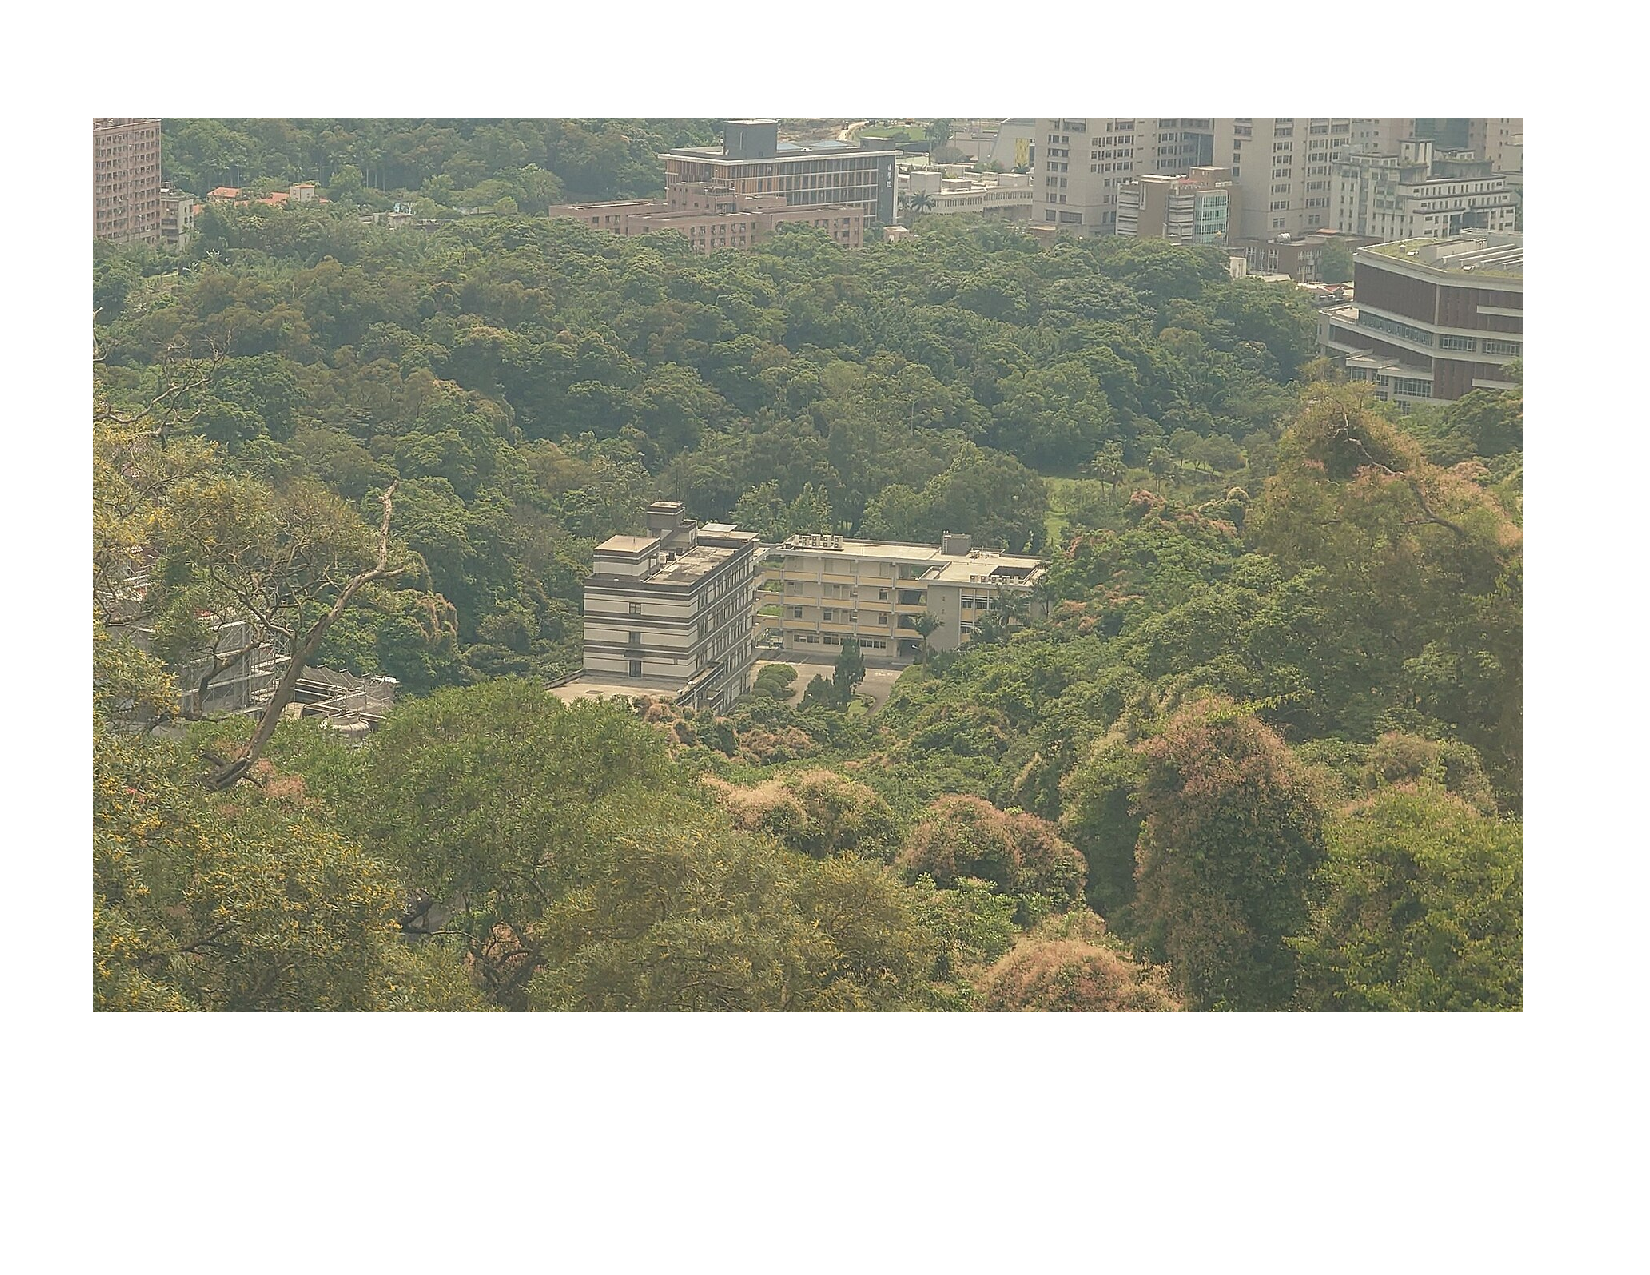
\includegraphics[width=0.8\linewidth]{Figs/nccu} \end{center}
\vspace{0.3cm}
\begin{center}
\small
Institute of International Relations, National Chengchi University (Taipei)
\end{center}
\end{frame}

\begin{frame}
\begin{itemize}
  \item From intelligence services to academic research
  \vspace{0.3cm}
  \item From area studies to comparative politics
  \vspace{0.1cm}
  \begin{itemize}
    \item Earlier generations of China scholars treat China as a distinct subfield within political science
    \item Later on, China scholars begin to borrow or "stretch" concepts and ideas from other subfields to study Chinese politics (Shambaugh 2023)
    \item Starting from the late 2000s, China scholars are about to generate new theoretical insights to general political science (Tsai 2017)
  \end{itemize}
  \vspace{0.3cm}
  \item From qualitative description to data-intensive inference
\end{itemize}
\end{frame}

\begin{frame}
\begin{center}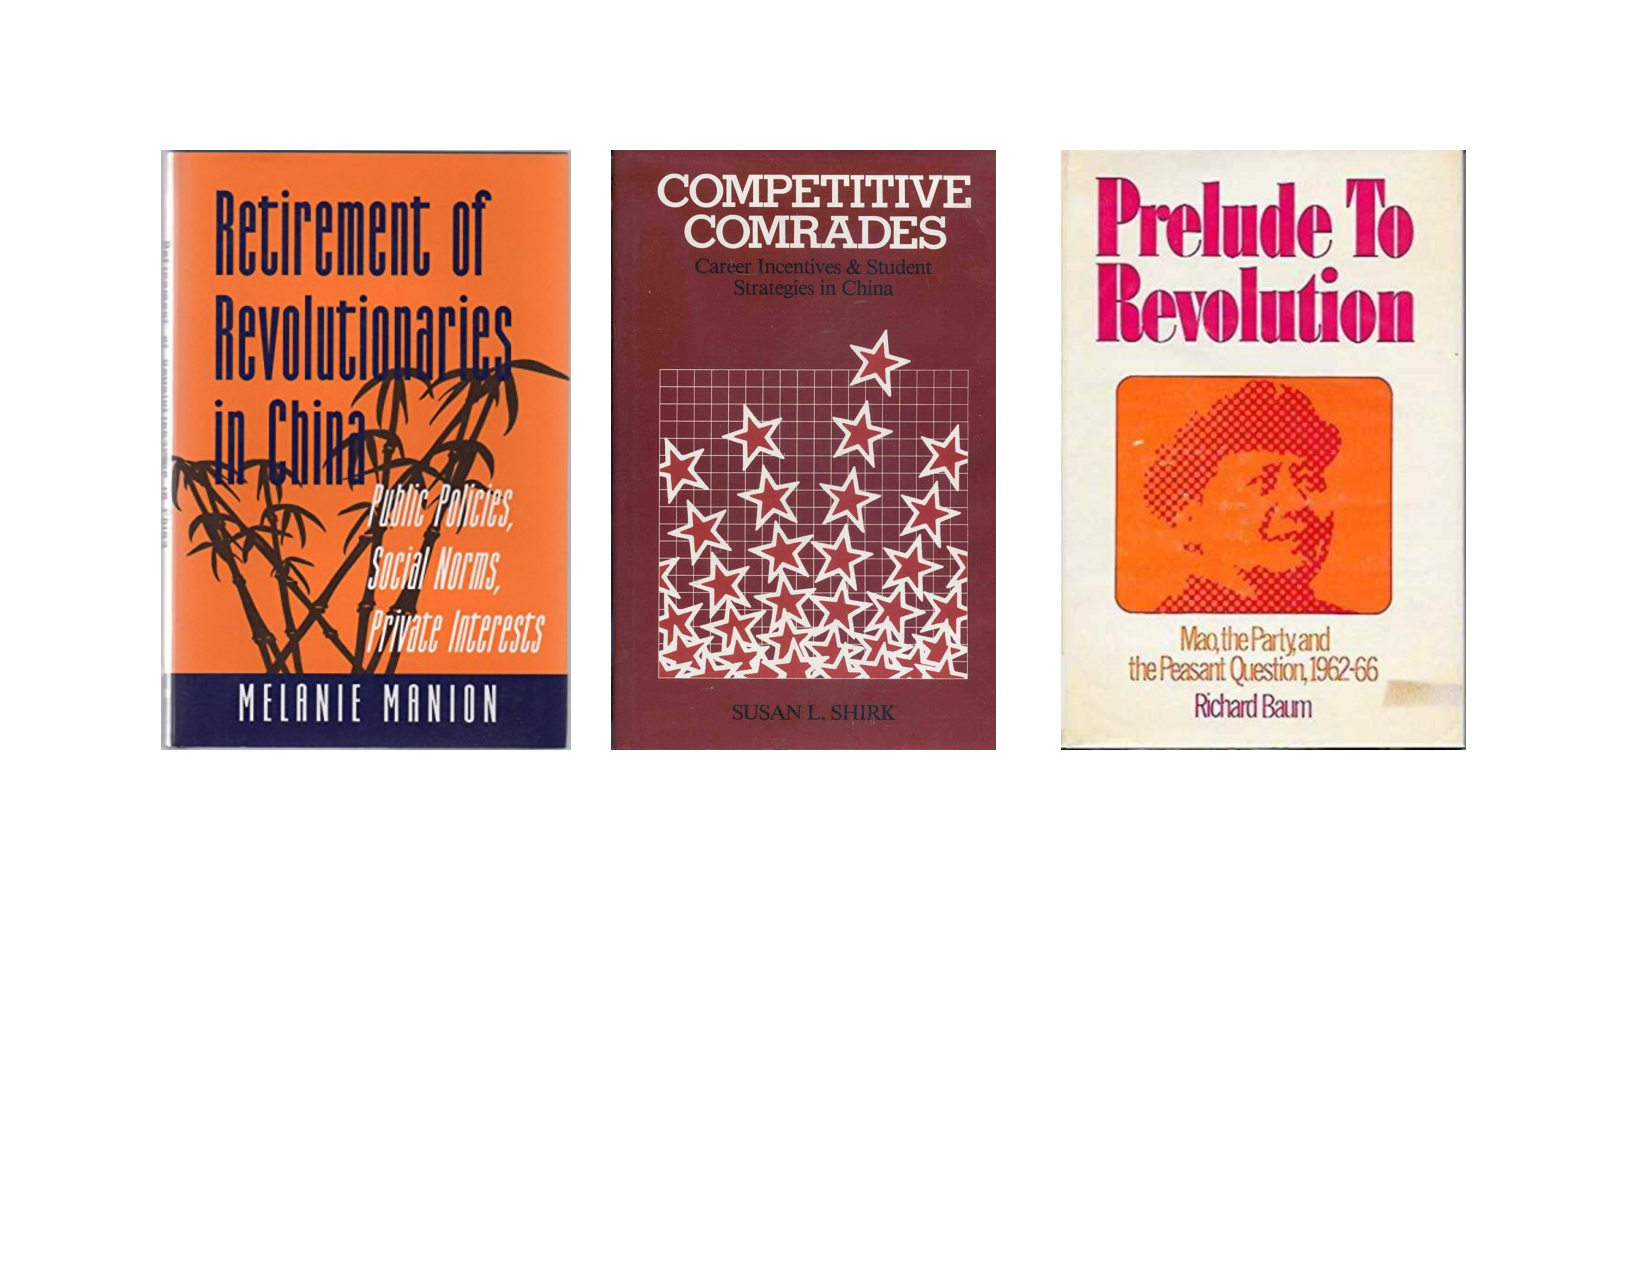
\includegraphics[width=1\linewidth]{Figs/book1} \end{center}
\end{frame}

\begin{frame}
\begin{center}\includegraphics[width=1\linewidth]{Figs/book2} \end{center}
\end{frame}

\begin{frame}
\begin{center}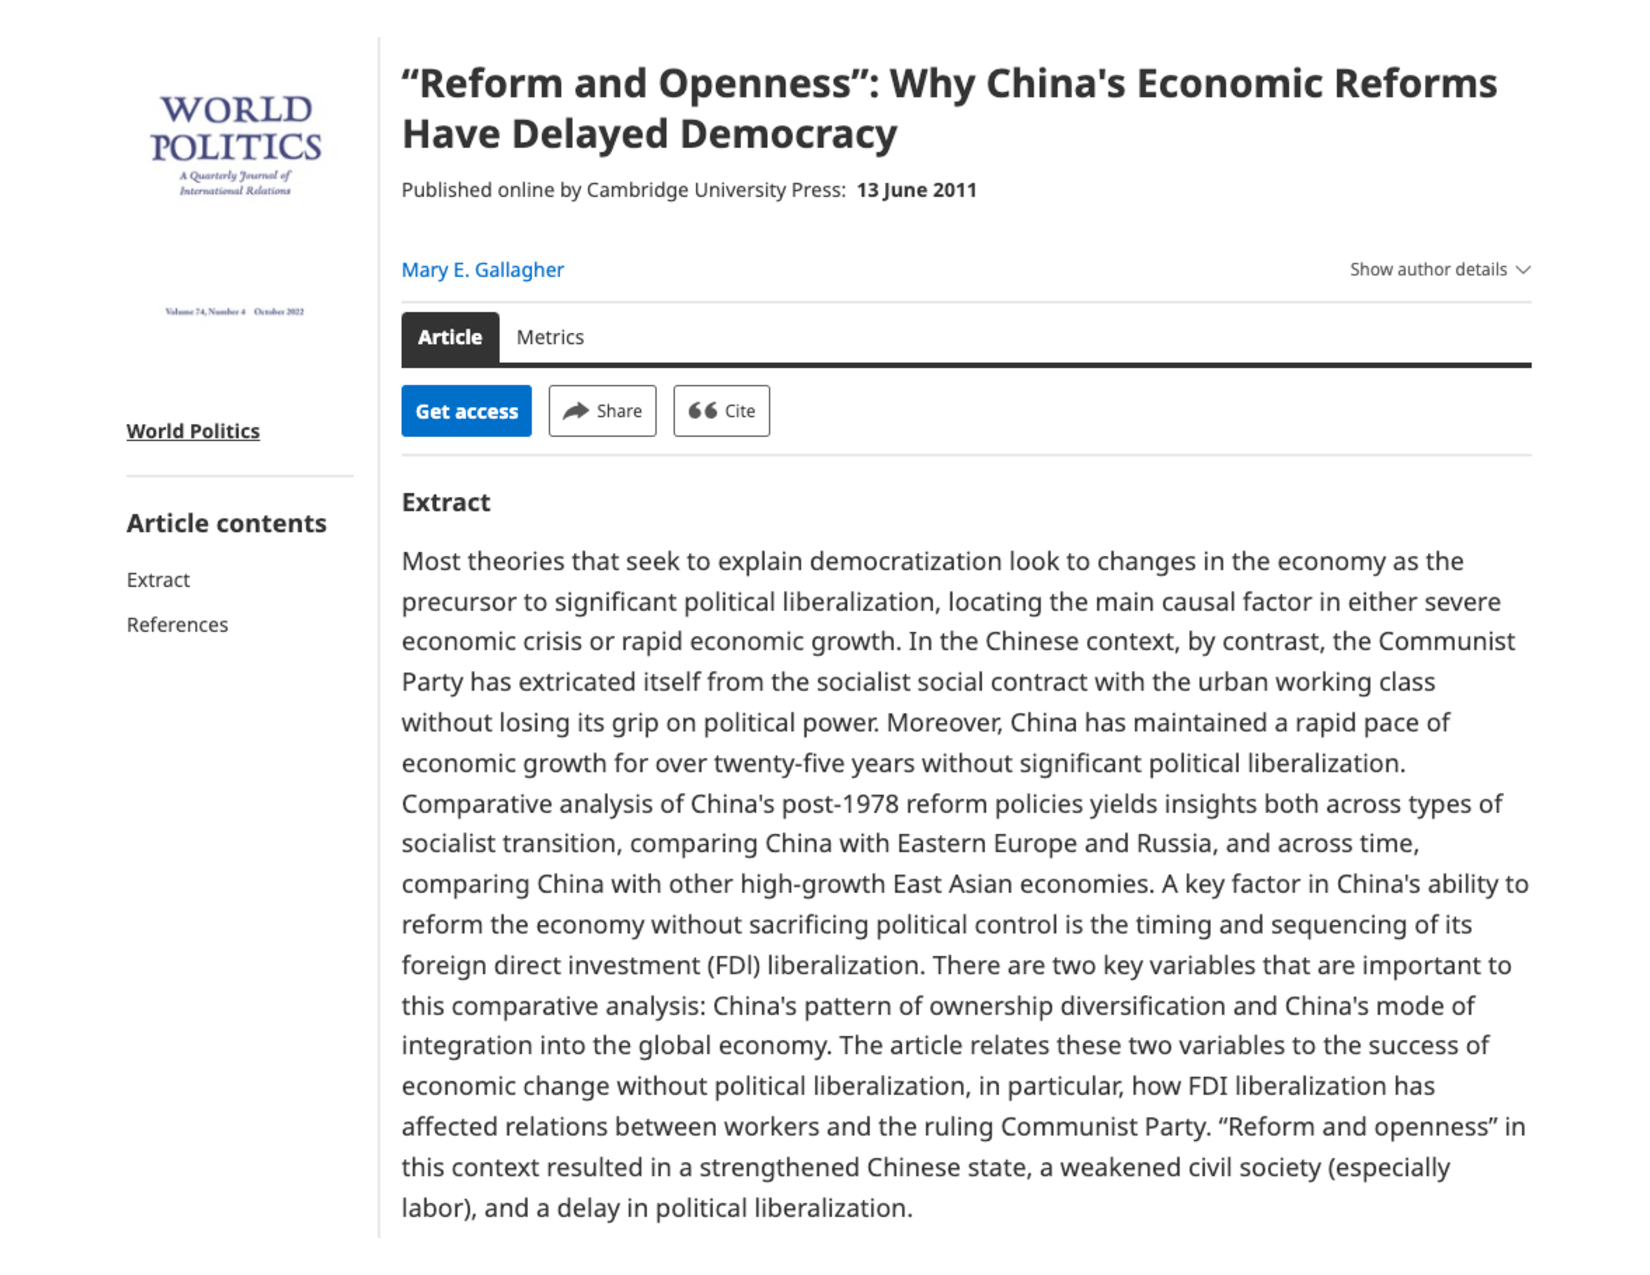
\includegraphics[width=1\linewidth]{Figs/mary} \end{center}
\end{frame}

\begin{frame}
\begin{center}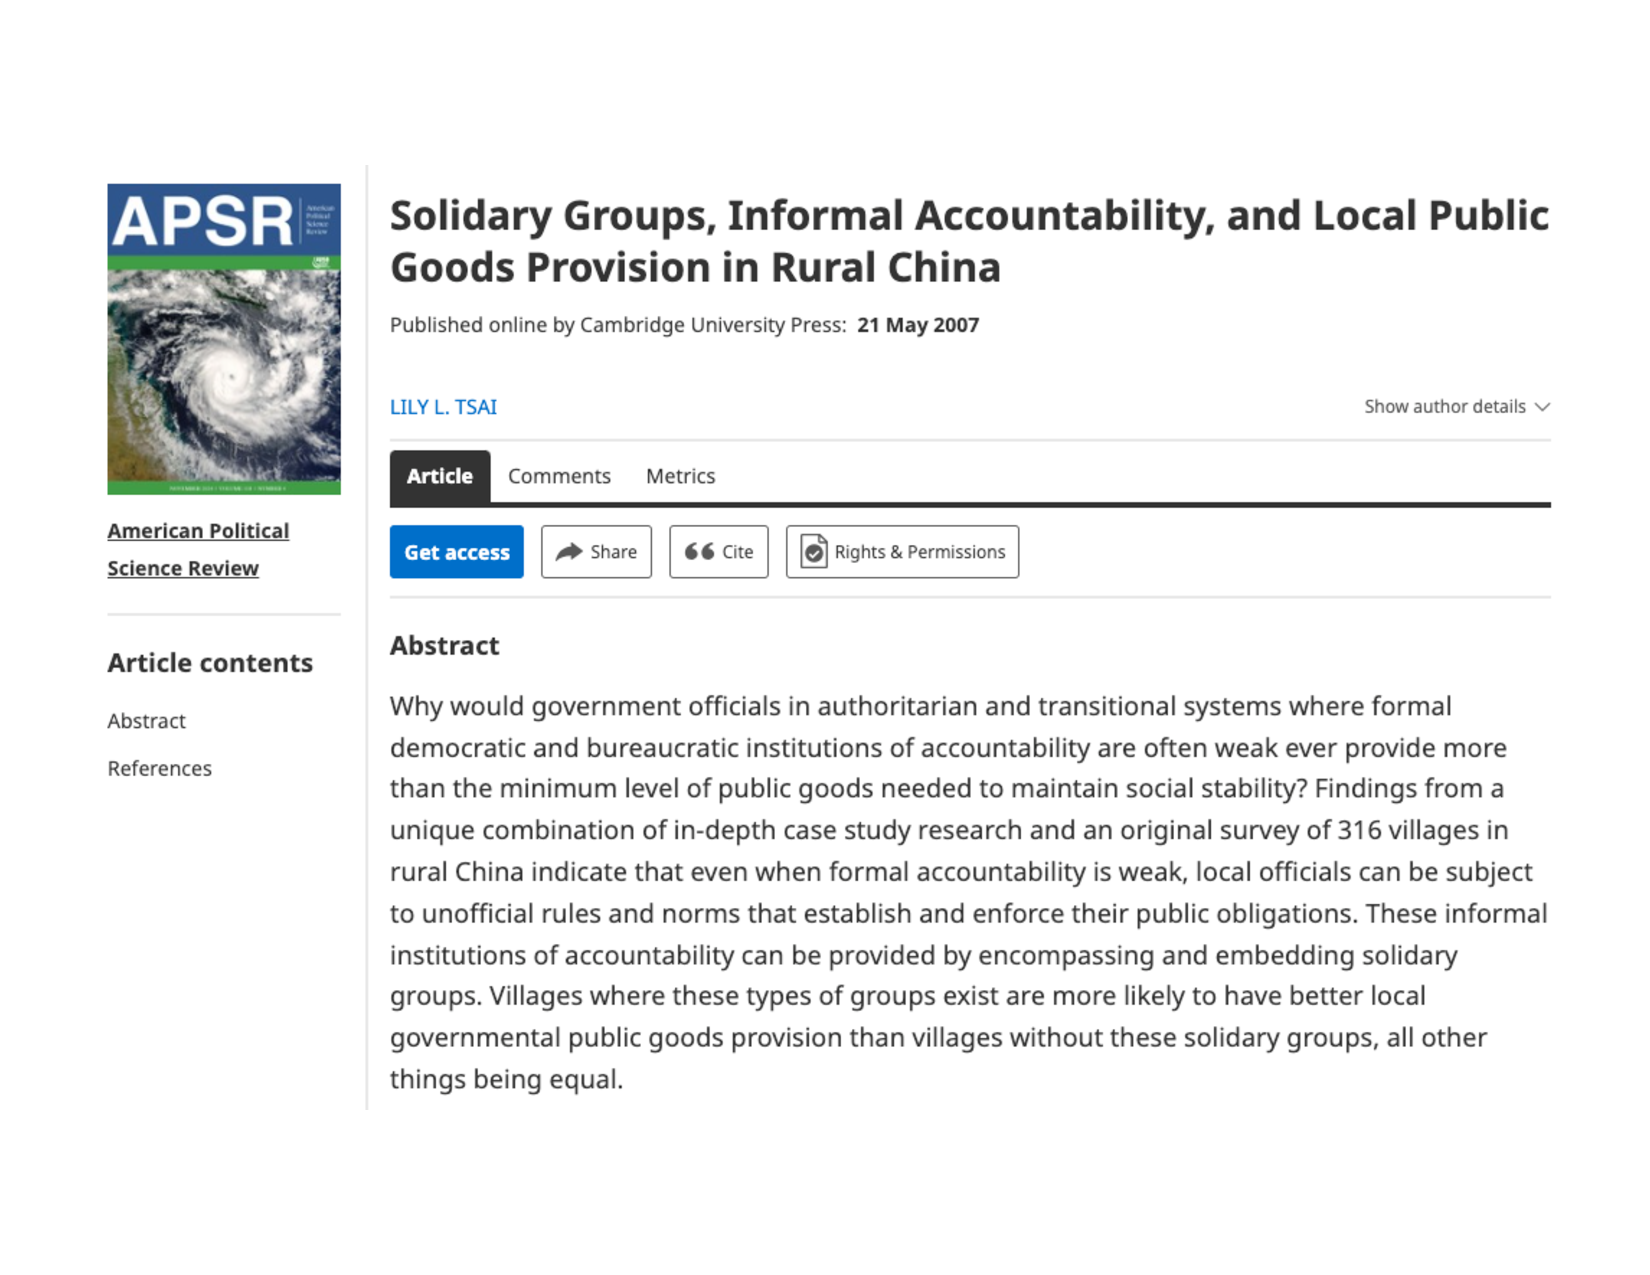
\includegraphics[width=1\linewidth]{Figs/tsai} \end{center}
\end{frame}

\begin{frame}
\begin{center}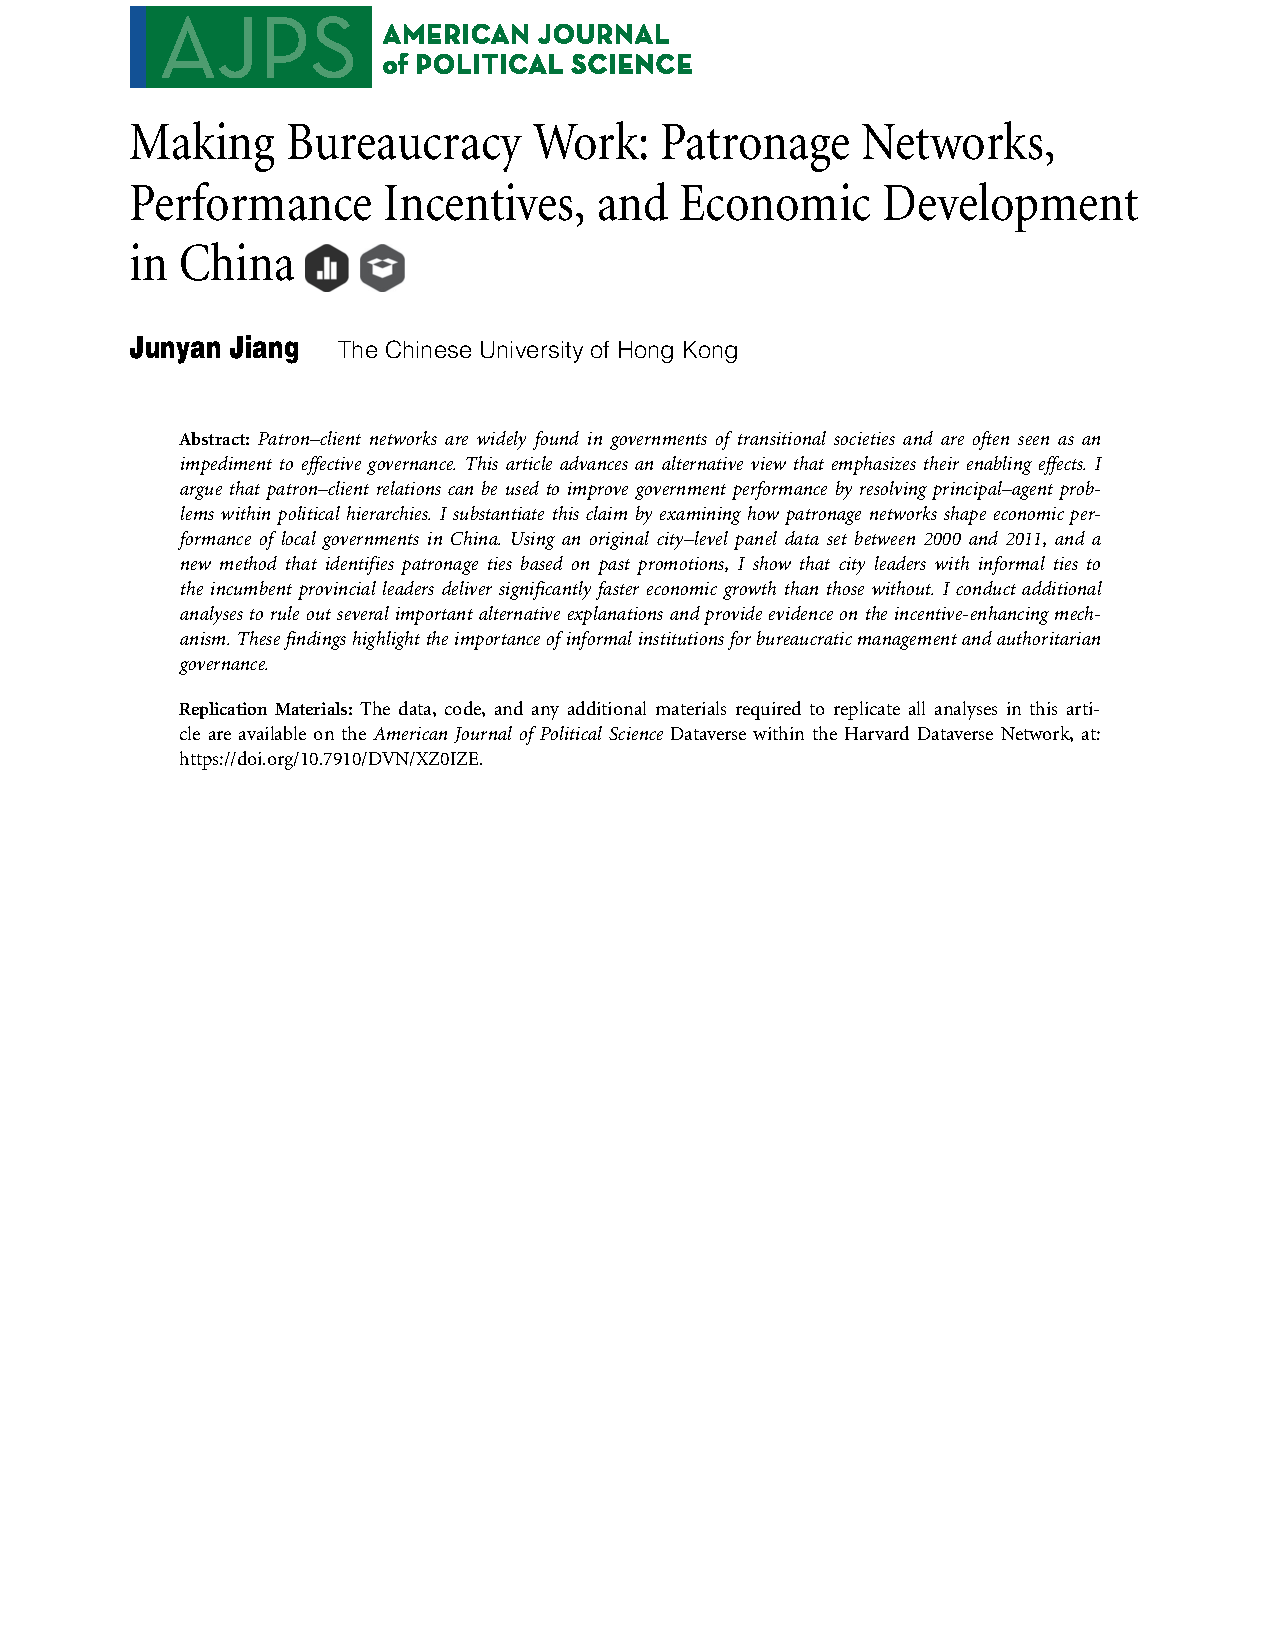
\includegraphics[width=0.95\linewidth]{Figs/jiang} \end{center}
\end{frame}

\begin{frame}
\begin{itemize}
  \item From intelligence services to academic research
  \vspace{0.3cm}
  \item From area studies to comparative politics
  \vspace{0.3cm}
  \item From qualitative description to data-intensive inference
  \vspace{0.1cm}
  \begin{itemize}
    \item Before the diplomatic reconciliation between PRC and USA (1971-1978), scholars have to rely on limited, parrial and often biased qualitative evidence (archives and interviews)
    \item After Reform and Opening, in the 1980s more engaging field research is likely (ethnography and case studies)
    \item The mid-1990s saw the quantitative turn of China studies (surveys, econometric analysis of admin data and computational)
  \end{itemize}
\end{itemize}
\end{frame}

\begin{frame}
\begin{center}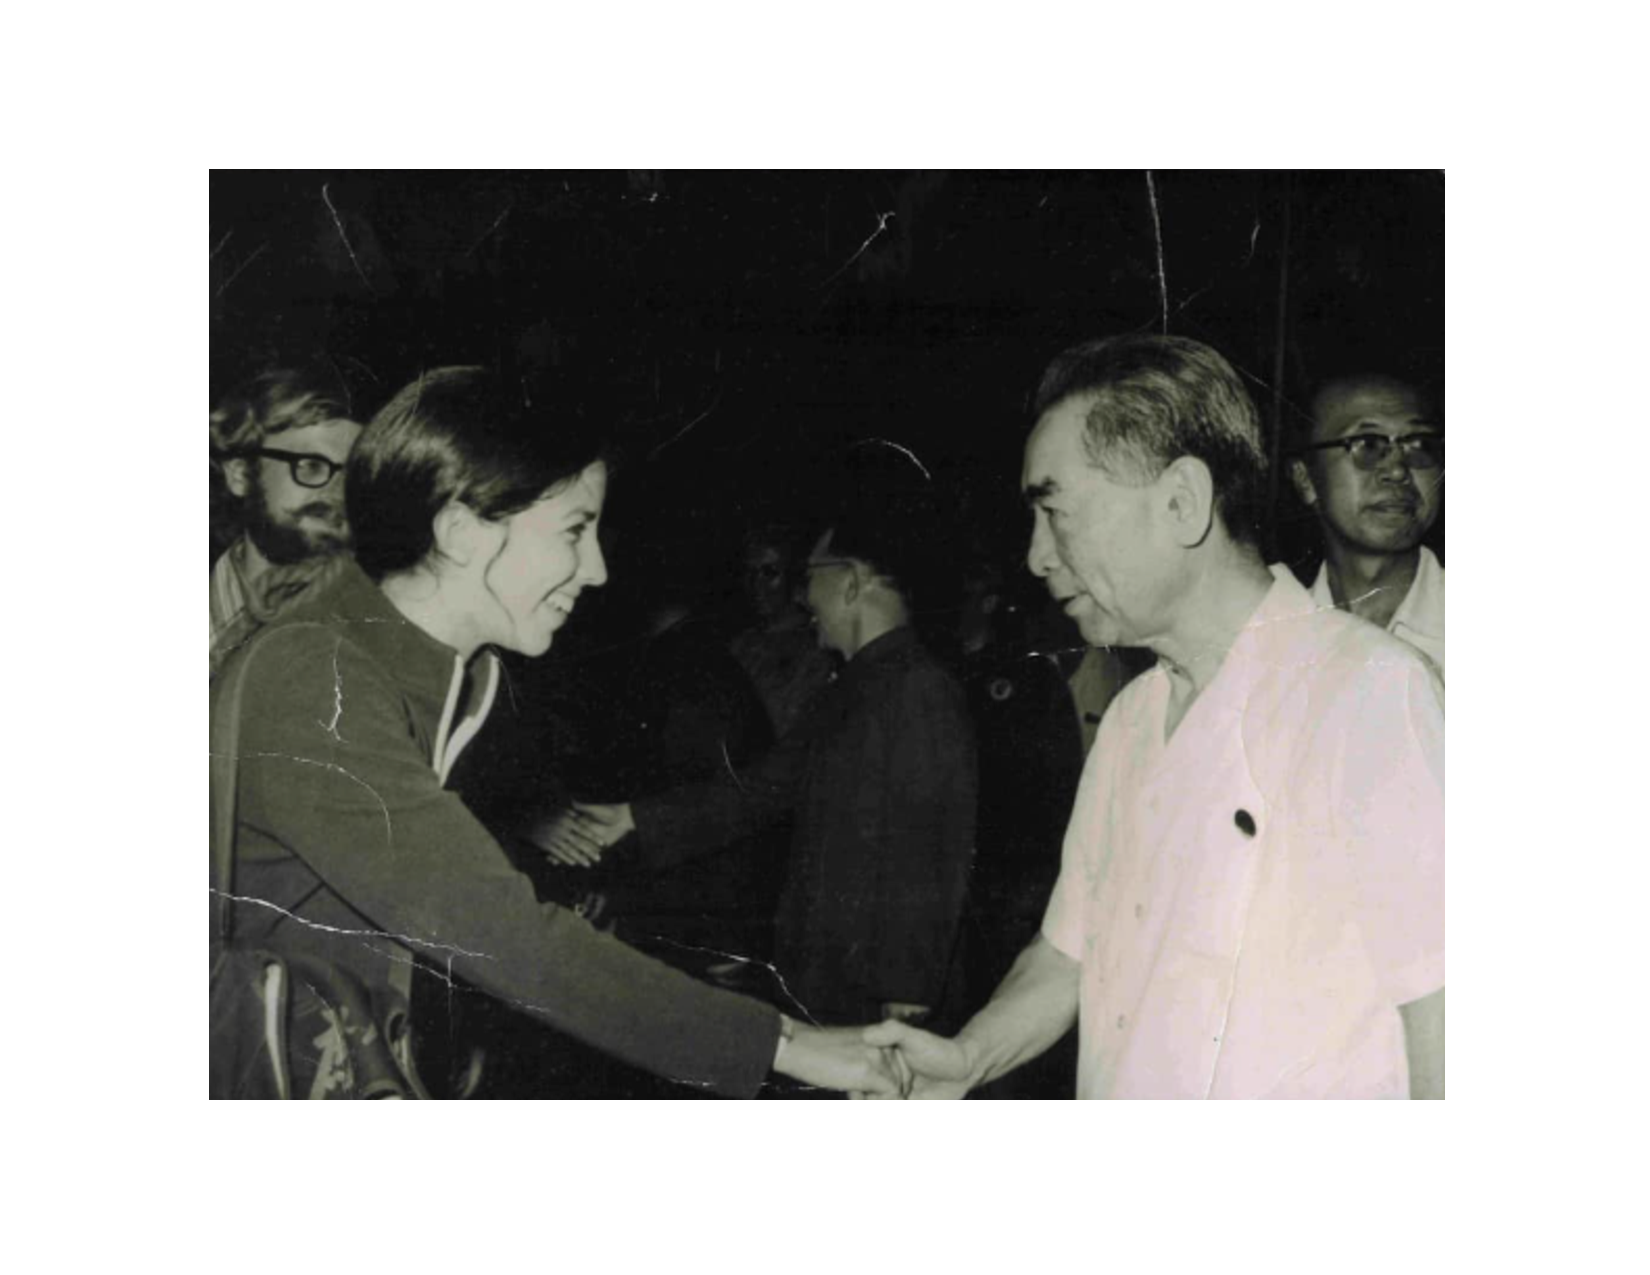
\includegraphics[width=0.9\linewidth]{Figs/shirk71} \end{center}
\vspace{0.1cm}
\begin{center}
\scriptsize
\small
Susan Shirk (UCSD) with Zhou Enlai in July 1971, on a visit to China with "the Committee of Concerned Asian Scholars"
\end{center}
\end{frame}

\begin{frame}
\begin{center}
\textbf{Week 2: Empire to Nation-State}
\end{center}
\vspace{0.3cm}

\begin{center}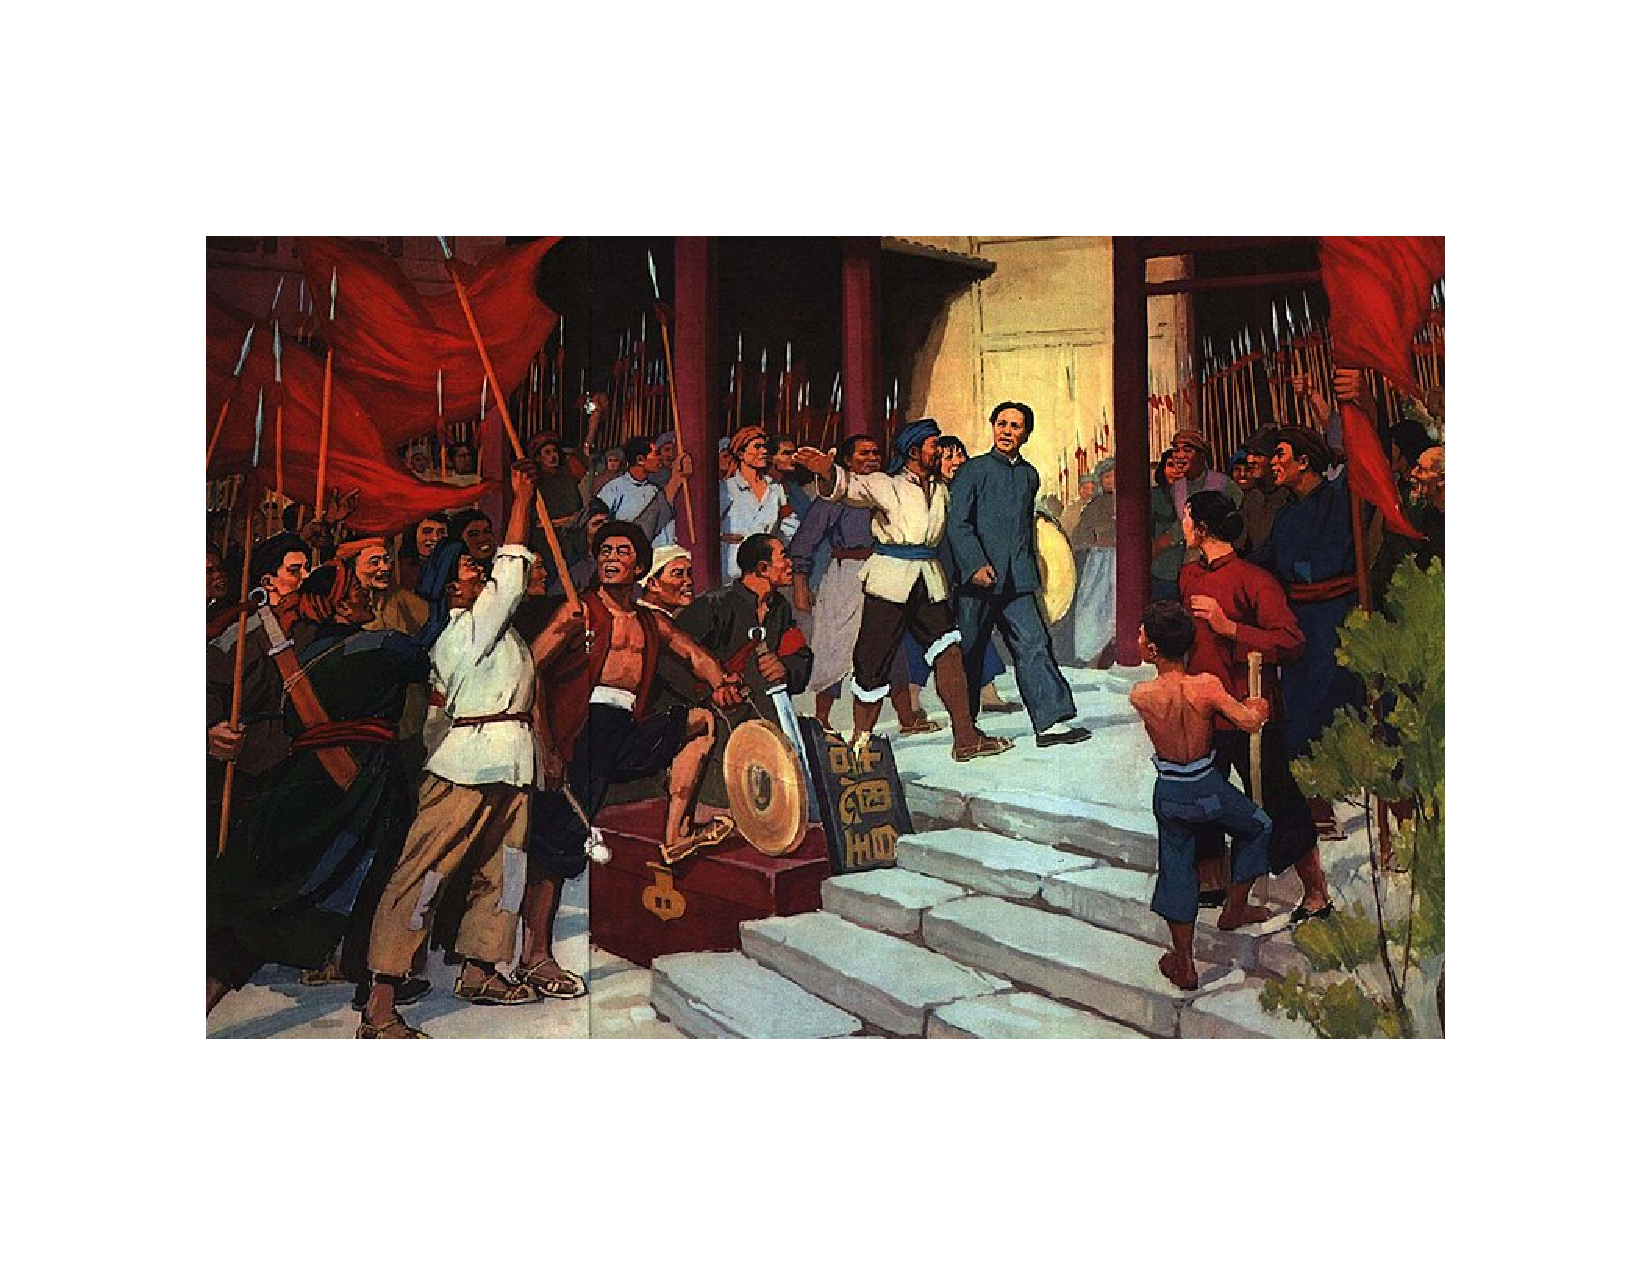
\includegraphics[width=0.7\linewidth]{Figs/theme2} \end{center}
\begin{center}
\footnotesize
\url{https://storystudio.tw/article/gushi/the-forbidden-garden}
\end{center}
\end{frame}

\begin{frame}{``China: A Century of Revolution''}
\protect\hypertarget{china-a-century-of-revolution}{}
\begin{center}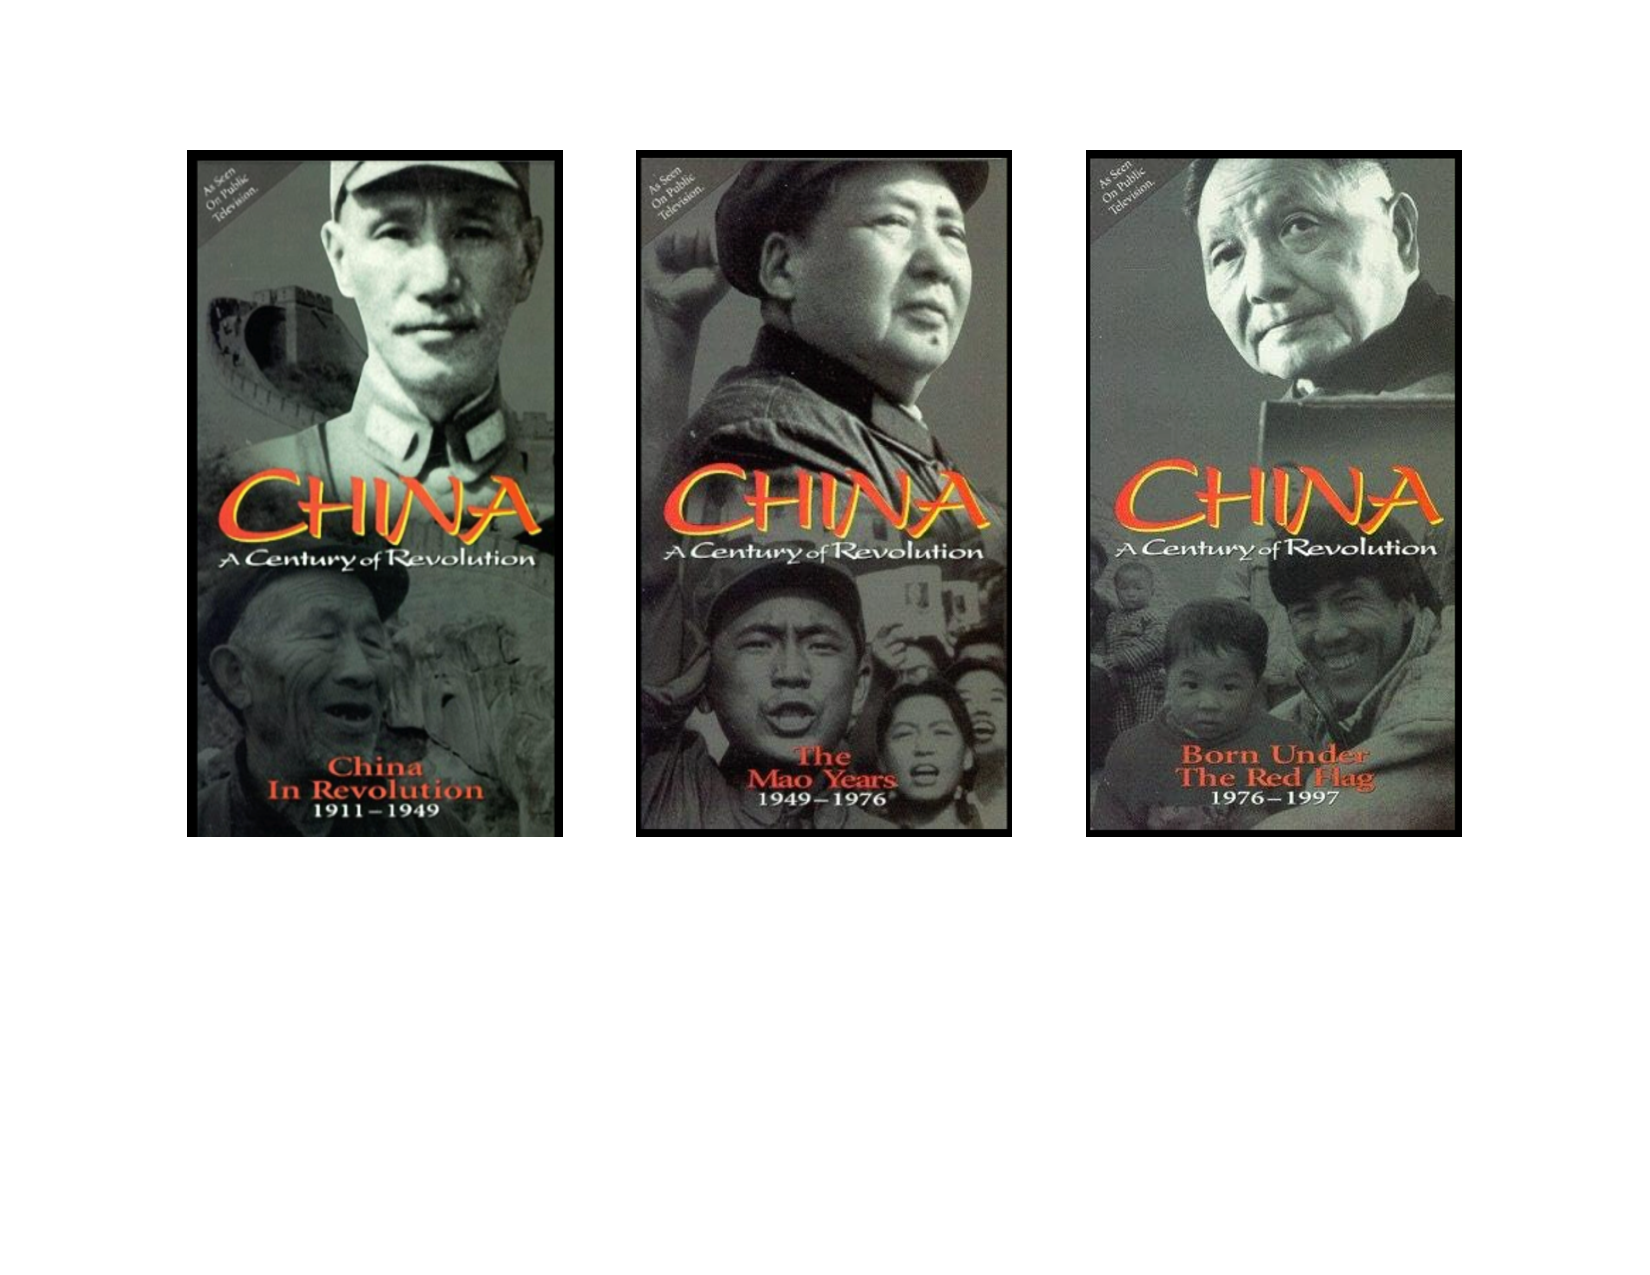
\includegraphics[width=0.95\linewidth]{Figs/docs} \end{center}
\end{frame}

\begin{frame}{China in the 20th century}
\protect\hypertarget{china-in-the-20th-century}{}
\begin{itemize}
  \item Republican China (1911-1949)
  \vspace{0.2cm}
  \begin{itemize}
    \item 1911-1928: Beiyang Government (北洋政府)
    \item 1928-1949: Nationalist/KMT Government (民国政府) 
  \end{itemize}
  \vspace{0.4cm}
  \item Communist China (1949 and afterwards)
  \vspace{0.2cm}
  \begin{itemize}
    \item 1950s: Land reform and the Great Leap Forward (大跃进)
    \item 1960s: Return of Mao Zedong and the outbreak of the Cultural Revolution (文化大革命)
    \item 1970s: Power transition and "Reform and Opening" (改革开放)
    \item 1980s: Experiment with market economy, intra-party split and Tiananmen
    \item 1990s: Consolidated market reform and institutionalized political succession
  \end{itemize}
\end{itemize}
\end{frame}

\begin{frame}{The pursuit of a ``modern'' China}
\protect\hypertarget{the-pursuit-of-a-modern-china}{}
\begin{itemize}
  \item Question: How do we define "modernity?"
  \pause
  \vspace{0.3cm}
  \item "Modernization" is a multi-dimensional concept
  \vspace{0.1cm}
  \begin{itemize}
    \item Political modernization: Transforming empire to centralized nation-state
    \item Social modernization: Filling the moral vacuum and searching for "new" ways of living (e.g., science, democracy and vernacular language and writing)
    \item Economic modernization: Industrial infrastructure and production (much of this has do with security threats)
  \end{itemize}
\end{itemize}
\end{frame}

\begin{frame}{Political modernization}
\protect\hypertarget{political-modernization}{}
TBA.
\end{frame}

\begin{frame}{Republican Era}
\protect\hypertarget{republican-era}{}
\begin{itemize}
  \item Beiyang period: Warlords and mass politics (urban students and intellectuals)
  \vspace{0.3cm}
  \item Nationalist period: CCP/CPC v GMD/KMT
  \vspace{0.1cm}
  \begin{itemize}
    \item GMD (KMT): Started as a revolutionary party rallying around Sun Ya-sen ("three principles of the people"); fraught with corruption and internal fragmentation
    \item CCP (CPC): Started as an urban party with the support from Comintern; relationship with GMD falling out and was forced (or struggled) to change and survive
  \end{itemize}
\end{itemize}
\end{frame}

\begin{frame}
\vspace{0.3cm}

\begin{center}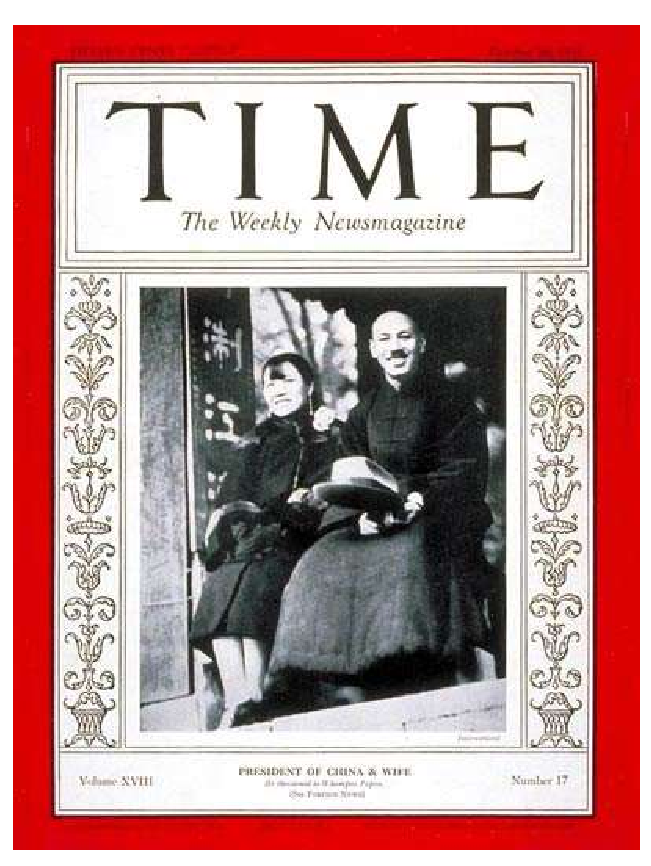
\includegraphics[width=0.5\linewidth]{Figs/chiang_new} \end{center}
\end{frame}

\begin{frame}
\vspace{0.3cm}

\begin{center}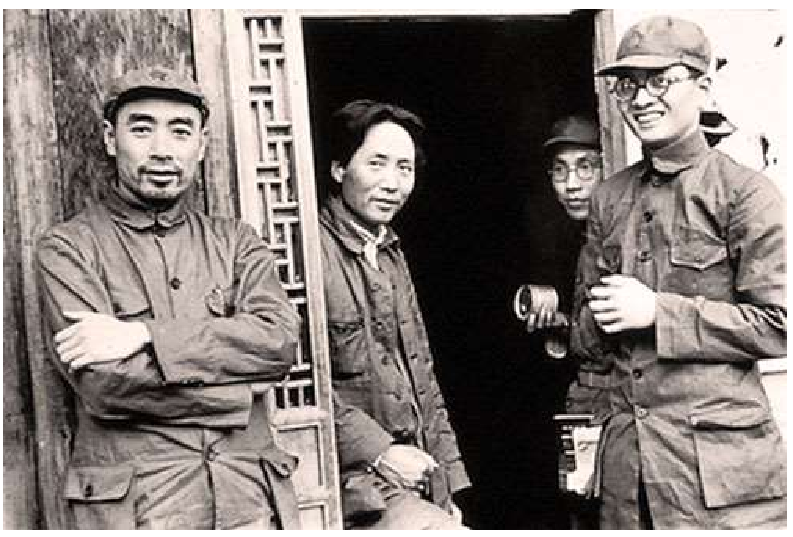
\includegraphics[width=0.9\linewidth]{Figs/yanan_new} \end{center}
\end{frame}

\begin{frame}
\vspace{0.3cm}

\begin{center}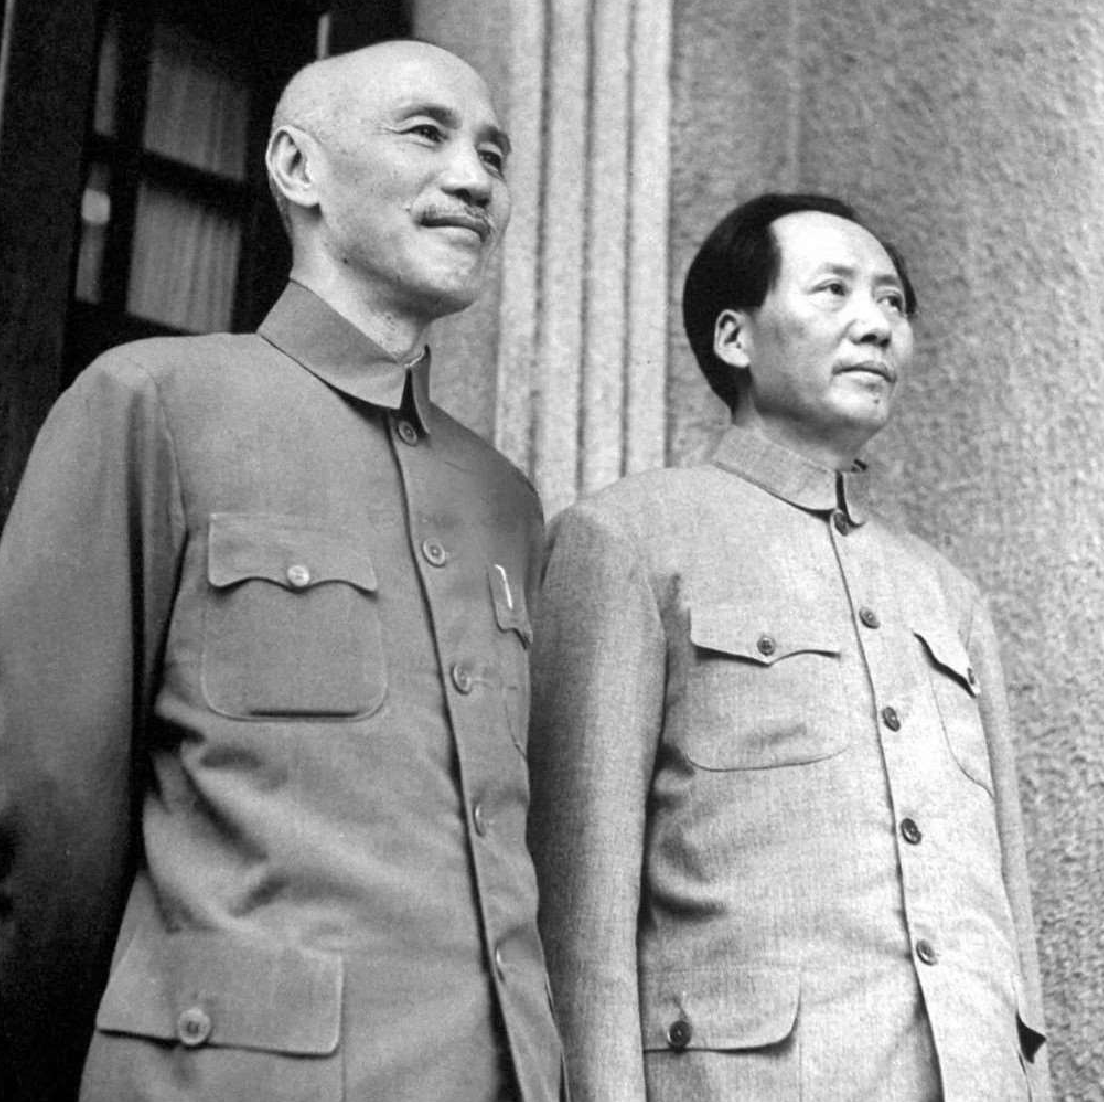
\includegraphics[width=0.6\linewidth]{Figs/chongqing_new} \end{center}
\end{frame}

\begin{frame}{The Chinese Civil War(s)}
\protect\hypertarget{the-chinese-civil-wars}{}
\begin{itemize}
  \item First Chinese Civil War (1927-1936)
  \begin{itemize}
    \item As a result of the fallout of the first United Front (1924-1927) duing the North Expedition; ended by the Xi'an Incident (西安事变)
    \item Key developments for GMD: The Nationalist Government managed to \textit{de facto} unify the country but Chiang Kai-shek was under constant challenges; industrial development took off in the shadow of Japanese invasion 
    \item Key developments for For CPC: The experiment with in Ruijin, Jiangxi
  \end{itemize}
  \vspace{0.3cm}
  \item Second Chinese Civil War (1945-1949)
  \begin{itemize}
    \item As a result of the end of WWII or the Anti-Japanese War (1937-1945); ended with the CPC's military victory
    \item The GMD's defeat was the result of its separation from its political and economic base (Lieberthal 1995)
  \end{itemize}
\end{itemize}
\end{frame}

\begin{frame}{Legacies of the Republican Era}
\protect\hypertarget{legacies-of-the-republican-era}{}
\begin{itemize}
  \item A divided "China:" CPC and GMD managed to control the Mainland China and Taiwan, respectively
  \vspace{0.6cm}
  \item CPC's revolutionary success against all odds
  \vspace{0.1cm}
  \begin{itemize}
    \item Grassroots mobilization and campaigns in the countryside
    \item Revolutionary armed forces
    \item Shared challenging experiences and collective memories
    \item Rise of Mao and the distance from the Soviet Union
    \item ...?
  \end{itemize}
\end{itemize}
\end{frame}

\begin{frame}{Local states in the early 20th century (Remick 2002)}
\protect\hypertarget{local-states-in-the-early-20th-century-remick-2002}{}
\begin{itemize}
  \item Key idea(s): The behavior and capacity of local states vary significantly in China, as these two are shaped by central policy and local social contexts (history, limitations and ideology)
  \vspace{0.3cm}
  \item Some questions to consider:
  \vspace{0.1cm}
  \begin{itemize}
    \item What is a state and state "capacity?" How did Remick define it? Why is state-building an important question? Why did she and many scholars choose to focus on taxation and public finance?
    \item Why do we need to look central and local state-building as two distinctive and yet interrelated processes?
    \item She mentioned a couple of countries to put her argument in a comparative perspective. Why? Does it make sense to you? Any other cases you can think of?
  \end{itemize}
\end{itemize}
\end{frame}

\begin{frame}{Concluding remarks: Questions remain for comparative
scholars}
\protect\hypertarget{concluding-remarks-questions-remain-for-comparative-scholars}{}
\begin{itemize}
  \item Revolutions: Causes, results and implications
  \vspace{0.3cm}
  \item Communist/Socialist revolutions and their influence
  \vspace{0.3cm}
  \item Political elites and leadership "style"
  \vspace{0.3cm}
  \item What else?
  \vspace{0.3cm}
  \item Opportunities and chanllenges: Why it is hard to study the early 20th century China: Taiwan, Hong Kong and Beijing
\end{itemize}
\end{frame}

\begin{frame}
Perry
\end{frame}

\begin{frame}
Ma and Ji
\end{frame}

\begin{frame}{Recap: Key events during the Republican Era}
\protect\hypertarget{recap-key-events-during-the-republican-era}{}
\begin{itemize}
  \item Beiyang period
  \vspace{0.1cm}
  \begin{itemize}
    \item 1919: May-Fourth Movement (五四运动)
    \item 1926-1928: North Expedition (北伐)
  \end{itemize}
  \vspace{0.3cm}
  \item Republican period
  \begin{itemize}
    \item 1927-1936: 1st CCP-GMD Civil War (一次国共内战)
    \item 1934-1935: Long March (长征) and Zunyi Conference (遵义会议)
    \item 1937-1945: Anti-Japanese War (抗日战争)
    \item 1942-1945: Rectification Movement (整风运动)
    \item 1945-1949: 2nd CCP-GMD Civil War (二次国共内战)
  \end{itemize}
\end{itemize}
\end{frame}

\begin{frame}
\vspace{1cm}

See you next week!
\end{frame}

\end{document}
